\documentclass[11pt,a4paper]{article}

\usepackage[utf8]{inputenc}
\usepackage[T1]{fontenc}
\usepackage[french]{babel}
\usepackage{lmodern}
\usepackage{microtype}
\usepackage[margin=2.3cm]{geometry}
\usepackage{booktabs}
\usepackage{tabularx}
\usepackage{array}
\usepackage{xcolor}
\usepackage{enumitem}
\usepackage{float}
\usepackage{graphicx}
\usepackage{amsmath}
\usepackage[round,authoryear]{natbib}
\usepackage[colorlinks=true,linkcolor=teal!70!black,citecolor=teal!70!black,urlcolor=teal!70!black]{hyperref}

\newcolumntype{Y}{>{\raggedright\arraybackslash}X}
\setlist{itemsep=2pt,topsep=4pt}

\title{\textbf{Livrable L3 -- Méthodes de référence}\\[4pt]
\large Allocation adaptative des ressources de calcul et de recherche documentaire\\ pour des systèmes LLM locaux, économes et fiables\\[2pt]
\normalsize\textit{Choix de la recherche documentaire, gel du protocole, routeurs de référence}}
\author{Alae Lahbichi -- Étudiant en 5\textsuperscript{e} année IA/Data\\[2pt]
\small\href{mailto:a.lahbichi2004@gmail.com}{\texttt{a.lahbichi2004@gmail.com}}\\
\small Dépôt GitHub : \href{https://github.com/AlaeLahbichi/Adaptive-Compute-and-RAG-for-Efficient-Reliable-Local-LLMs}{\footnotesize\texttt{AlaeLahbichi/Adaptive-Compute-and-RAG-for-Efficient-Reliable-Local-LLMs}}}
\date{18 octobre 2026}

\begin{document}
\maketitle

\begin{abstract}
\noindent Cette partie construit les adversaires que la méthode adaptative (Partie IV) devra battre.
D'abord, trois méthodes de recherche documentaire sont comparées sur le jeu de développement. La
recherche lexicale BM25 l'emporte nettement sur la recherche dense du pilote : son rappel@3 passe de
0,60 à 0,82 sur les questions simples et de 0,22 à 0,37 sur les questions complexes, et elle est 40 fois
plus rapide. Elle est retenue, et le protocole est gelé (étiquette \texttt{protocole-v1.0}). Ensuite,
six stratégies fixes (A à F) sont exécutées, puis deux routeurs de référence fondés sur le seul texte de
la question sont évalués par validation croisée : un routeur coût--qualité qui choisit parmi les six
stratégies (R1, contrôle exigé par la revue L1) et une version simplifiée d'Adaptive-RAG (R2).
Avec la recherche BM25, la référence B (grand modèle + 3 passages) passe de 0,42 à 0,54 de score
global. Aucun des deux routeurs ne satisfait le critère principal. R1, au réglage 20\,\% plus rapide que
B, perd 11,6 points ; R2 reste proche de B en qualité ($-1{,}9$ point) mais ne gagne que 8\,\% de
latence. Un routeur parfait (oracle) atteindrait pourtant 0,76 en 0,40~s. Lire la seule question ne
suffit donc pas : il faut des signaux plus informatifs, ce que la Partie IV devra apporter.
\end{abstract}

\clearpage
\tableofcontents
\clearpage

%======================================================================
\section{Rôle de cette partie}
%======================================================================

Une méthode ne se juge qu'à l'aune de ce qui existe déjà. La Partie II a fixé l'épreuve (questions,
métriques, critères de succès) ; la Partie III installe des \emph{concurrents de référence} sérieux,
pour qu'un éventuel gain de la Partie IV ne puisse pas être attribué à des comparaisons trop faciles.
Trois objectifs :
\begin{enumerate}
\item \textbf{Fixer la recherche documentaire}, maillon faible relevé au pilote, puis geler le protocole.
\item \textbf{Mesurer ce qu'obtient un routeur qui ne lit que la question} (R1). La revue L1 a montré que
des signaux plus coûteux n'apportent souvent rien de plus qu'un tel contrôle \citep{li2026beyond}.
\item \textbf{Reproduire le travail publié le plus proche}, Adaptive-RAG \citep{jeong2024adaptiverag},
sous une forme simplifiée et dans nos conditions (R2).
\end{enumerate}
Tout est réglé et évalué sur le \textbf{jeu de développement} (180 questions). Le jeu de test reste
intact.

%======================================================================
\section{Choix de la recherche documentaire}\label{sec:recherche}
%======================================================================

\paragraph{Méthodes comparées.}
\begin{itemize}
\item \textbf{Dense} (pilote) : embeddings MiniLM et similarité cosinus, qui compare le \emph{sens}.
\item \textbf{BM25} : score lexical Okapi ($k_1 = 1{,}5$, $b = 0{,}75$, mots vides retirés), qui compare
les \emph{mots} ; implémenté directement avec une matrice creuse.
\item \textbf{Hybride} : fusion des deux classements par la somme des inverses des rangs
(\textit{Reciprocal Rank Fusion}, constante 60).
\end{itemize}

\begin{table}[H]
\centering\small
\begin{tabular}{l c c c c c c c}
\toprule
& \multicolumn{3}{c}{\textbf{Simple}} & \multicolumn{3}{c}{\textbf{Complexe}} & \\
\cmidrule(lr){2-4}\cmidrule(lr){5-7}
\textbf{Méthode} & @1 & @3 & @6 & @1 & @3 & @6 & \textbf{Temps / requête} \\
\midrule
Dense   & 0,48 & 0,60 & 0,70 & 0,00 & 0,22 & 0,35 & 7,4 ms \\
\textbf{BM25} & \textbf{0,65} & \textbf{0,82} & \textbf{0,87} & 0,00 & \textbf{0,37} & \textbf{0,50} & \textbf{0,2 ms} \\
Hybride & 0,60 & 0,72 & 0,80 & 0,00 & 0,33 & 0,48 & 7,1 ms \\
\bottomrule
\end{tabular}
\caption{Rappel de la recherche sur le jeu de développement (60 questions par catégorie). Pour une
question complexe, les deux passages justificatifs doivent être récupérés : le rappel@1 est donc nul
par construction. Questions non couvertes (rappel du paragraphe d'origine, @1 / @3 / @6) : dense 0,52 /
0,68 / 0,77 ; BM25 0,73 / 0,83 / 0,87 ; hybride 0,65 / 0,90 / 0,97.}
\label{tab:recherche}
\end{table}

\paragraph{Décision.} BM25 est retenu. Sur les questions qui ont une réponse (simples et complexes),
il domine les deux autres méthodes à chaque profondeur, tout en étant 40 fois plus rapide et sans
modèle d'embeddings à exécuter. Sur les questions non couvertes, la recherche hybride retrouve plus
souvent le paragraphe d'origine (rappel@3 de 0,90 contre 0,83). Ce critère compte moins pour elles, car
le comportement attendu est de s'abstenir et le paragraphe d'origine ne contient pas la réponse. Ce résultat s'explique par la
nature des questions, riches en noms propres et en termes repris du texte source, et par la faiblesse
relative du petit modèle d'embeddings multilingue. La fusion hybride, à poids égaux, est tirée vers le
bas par la composante dense.

\paragraph{Gel du protocole.} Le fichier \texttt{configs/protocole\_v1.json} (version 1.0) consigne ce
choix ainsi que deux stratégies supplémentaires à 6 passages, E et F, qui complètent l'espace de
décision annoncé dans L2. L'étiquette Git \texttt{protocole-v1.0} fige cet état. Les empreintes des
données (\texttt{MANIFEST.json}) sont inchangées depuis L2.

%======================================================================
\section{Les six stratégies fixes avec la recherche BM25}\label{sec:strategies}
%======================================================================

\begin{table}[H]
\centering\footnotesize\setlength{\tabcolsep}{4pt}
\begin{tabular}{l c c c c c c c c}
\toprule
\textbf{Stratégie} & \textbf{Score} & \textbf{IC 95\,\%} & \textbf{Simple} & \textbf{Complexe} & \textbf{Non couv.} & \textbf{Couv.} & \textbf{Risque} & \textbf{Latence} \\
\midrule
A -- grand, 0 passage   & 0,312 & [0,248 ; 0,378] & 0,07 & 0,09 & 0,78 & 0,31 & 0,82 & 0,25 s \\
B -- grand, 3 passages  & \textbf{0,541} & [0,472 ; 0,610] & 0,68 & 0,36 & 0,58 & 0,62 & 0,39 & 0,92 s \\
C -- petit, 0 passage   & 0,233 & [0,174 ; 0,294] & 0,05 & 0,07 & 0,58 & 0,46 & 0,93 & 0,13 s \\
D -- petit, 3 passages  & 0,330 & [0,267 ; 0,397] & 0,48 & 0,29 & 0,22 & 0,83 & 0,69 & 0,37 s \\
E -- grand, 6 passages  & 0,570 & [0,501 ; 0,637] & 0,70 & 0,45 & 0,57 & 0,67 & 0,40 & 1,63 s \\
F -- petit, 6 passages  & 0,372 & [0,308 ; 0,439] & 0,53 & 0,37 & 0,22 & 0,89 & 0,66 & 0,62 s \\
\bottomrule
\end{tabular}
\caption{Stratégies fixes avec la recherche BM25 (jeu de développement, 180 questions). Les colonnes
Simple, Complexe et Non couv. donnent le score global par catégorie.}
\label{tab:strategies}
\end{table}

\paragraph{Effet du changement de recherche (par rapport au pilote de L2).} Les stratégies avec RAG
progressent nettement : B passe de 0,424 à 0,541 (+11,7 points) et devient un peu plus rapide (0,99 à
0,92~s), car BM25 coûte moins cher que l'encodage de la question. D passe de 0,298 à 0,330. Les
stratégies sans recherche (A, C) sont inchangées, comme attendu. La référence des critères de succès
est donc \emph{plus exigeante} qu'au pilote.

\paragraph{Six passages plutôt que trois.} E améliore B de 2,9 points, surtout sur les questions
complexes (0,45 contre 0,36), mais coûte 76\,\% de latence en plus. L'écart avec B n'est pas
significatif (IC 95\,\% de la différence : $[-1{,}1 ; +7{,}1]$ points). Une recherche plus large n'est
donc utile que pour une partie des questions, ce qui justifie de la décider question par question.

%======================================================================
\section{Routeurs de référence}\label{sec:routeurs}
%======================================================================

\subsection{Principe commun}
Les deux routeurs ne lisent \emph{que le texte de la question}, sans générer ni rechercher au préalable.
Leurs caractéristiques sont un TF-IDF sur les mots et les paires de mots, complété de quelques
indicateurs simples (longueur, nombre de mots en majuscule, présence de chiffres, de « and » ou
« both », mot interrogatif initial). Comme la génération est déterministe, la réponse d'un routeur à une
question est celle de la stratégie qu'il choisit, déjà calculée en section~\ref{sec:strategies}. Le temps
de calcul du routeur est mesuré et ajouté à la latence.

\paragraph{Validation croisée.} Avec 180 questions, les routeurs sont entraînés et évalués par
validation croisée en 5 plis stratifiés par catégorie : chaque question est routée par un modèle qui ne
l'a jamais vue. Les résultats restent toutefois \emph{optimistes} : les hyperparamètres et le point de
fonctionnement de R1 sont choisis sur ce même jeu de développement. Seule l'évaluation finale sur le jeu
de test donnera une mesure non biaisée.

\subsection{R1 -- Routeur « question seule » (contrôle)}
Pour chaque stratégie $s \in \{A,\dots,F\}$, une régression ridge prédit le score $\hat{y}_s(q)$ à
partir de la question $q$. Le routeur choisit
\[
s^\star(q) = \arg\max_s \; \hat{y}_s(q) - \lambda \, \bar{t}_s ,
\]
où $\bar{t}_s$ est la latence moyenne de la stratégie $s$ sur les plis d'apprentissage. Le paramètre
$\lambda \geq 0$ règle le compromis : $\lambda = 0$ privilégie la qualité, un grand $\lambda$ privilégie
la vitesse. On fait varier $\lambda$ pour tracer une courbe qualité--coût, dans l'esprit de Hybrid LLM
\citep{ding2024hybrid}. Le point rapporté est le meilleur score parmi les réglages au moins 20\,\% plus
rapides que B, c'est-à-dire ceux qui satisfont la contrainte de latence du critère principal.

\subsection{R2 -- Adaptive-RAG simplifié}
Comme dans \citet{jeong2024adaptiverag}, un classifieur de complexité choisit, avec un modèle fixe (le
grand), entre aucune recherche (A), une recherche de 3 passages (B) et une recherche complémentaire de
6 passages (E). L'étiquette d'apprentissage d'une question est la stratégie la plus simple qui répond
correctement. Si aucune ne répond correctement, on reprend le biais par jeu de données de l'article
original : B pour SQuAD (une étape), E pour HotpotQA (plusieurs étapes). Le classifieur est une
régression logistique multinomiale. Deux simplifications par rapport à l'original sont assumées :
le classifieur est linéaire au lieu d'un modèle T5 affiné, et la recherche itérative est remplacée
par une recherche unique plus large.

%======================================================================
\section{Résultats}\label{sec:resultats}
%======================================================================

\begin{table}[H]
\centering\footnotesize\setlength{\tabcolsep}{3.5pt}
\begin{tabular}{l c c c c c c c}
\toprule
\textbf{Méthode} & \textbf{Score} & \textbf{Écart à B} & \textbf{IC 95\,\%} & \textbf{Latence} & \textbf{Gain vs B} & \textbf{Couv.} & \textbf{Risque} \\
\midrule
B -- référence & 0,541 & -- & -- & 0,92 s & -- & 0,62 & 0,39 \\
R1 -- question seule & 0,425 & $-11{,}6$ & $[-18{,}5 ; -4{,}8]$ & 0,74 s & 20\,\% & 0,58 & 0,57 \\
R2 -- Adaptive-RAG simplifié & 0,522 & $-1{,}9$ & $[-7{,}4 ; +3{,}3]$ & 0,85 s & 8\,\% & 0,49 & 0,39 \\
\textit{Oracle (A--F)} & \textit{0,762} & $+22{,}1$ & $[+16{,}5 ; +27{,}8]$ & \textit{0,40 s} & \textit{56\,\%} & 0,58 & 0,19 \\
\bottomrule
\end{tabular}
\caption{Routeurs de référence, validation croisée en 5 plis sur le jeu de développement. Surcoût de
calcul des routeurs inclus dans la latence : 0,5~ms pour R1, 0,3~ms pour R2. Écarts en points de score ; R1 au réglage $\lambda = 0{,}113$.}
\label{tab:routeurs}
\end{table}

\begin{figure}[H]
\centering
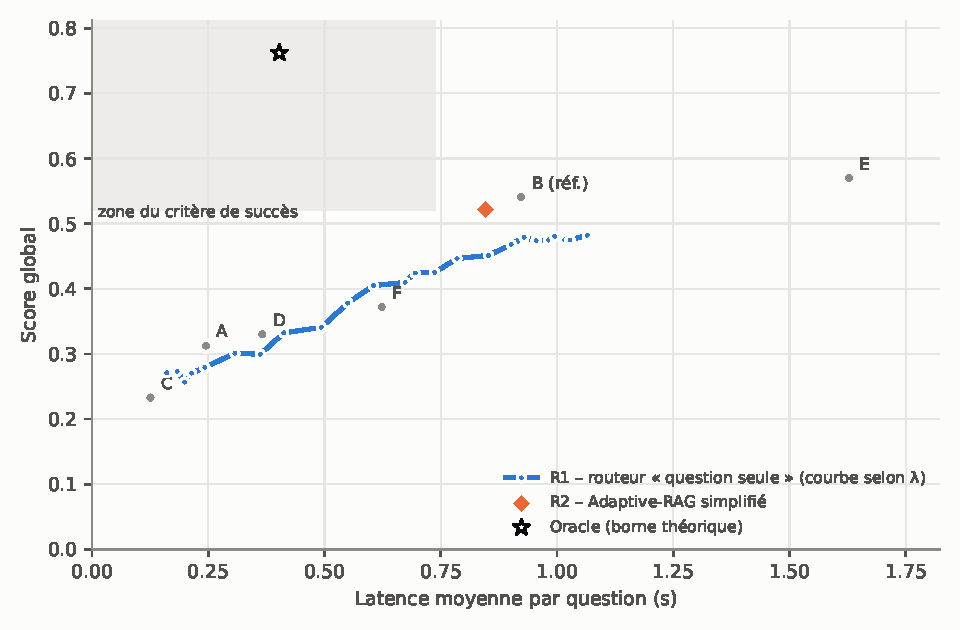
\includegraphics[width=0.92\textwidth]{figures/partie3_qualite_cout.pdf}
\caption{Compromis qualité--coût sur le jeu de développement. Points gris : stratégies fixes. Courbe
bleue : R1 pour 26 valeurs de $\lambda$. Losange orange : R2. Étoile : oracle. La zone grisée correspond
au critère principal : au moins 20\,\% plus rapide que B, pour au plus 2 points de score en moins.}
\label{fig:qualite-cout}
\end{figure}

\paragraph{R1 ne fait pas mieux que toujours choisir B.} Même au réglage qui privilégie la qualité
($\lambda = 0$), R1 n'atteint que 0,48, soit moins que B (0,54), pour une latence supérieure. Dès qu'on
lui impose d'être 20\,\% plus rapide, il perd 11,6 points. Sur ce benchmark, le texte de la question ne
permet pas de prédire de façon fiable quelle stratégie réussira. Une explication plausible, qui reste à
vérifier, est que la réussite dépend surtout de ce que contient le corpus et de ce que sait le modèle,
deux informations que la question seule ne révèle pas.

\paragraph{R2 garde la qualité de B, mais gagne peu de temps.} En choisissant entre 0, 3 et 6 passages,
R2 obtient 0,522, à moins de 2 points de B (écart non significatif), pour 8\,\% de latence en moins.
Il économise du temps en répondant sans recherche à 38 questions, dont il est d'ailleurs bon juge pour
les questions non couvertes (0,73 contre 0,58 pour B). En revanche, son classifieur de complexité ne
prédit la bonne étiquette que dans 42\,\% des cas, et il ne choisit jamais le petit modèle : son gain de
coût est donc plafonné.

\paragraph{La marge reste très grande.} L'oracle montre qu'en choisissant la bonne stratégie pour
chaque question, on pourrait à la fois améliorer le score de 22 points et diviser la latence par plus
de deux. Les deux routeurs n'en captent presque rien.

%======================================================================
\section{Ce que la méthode adaptative devra démontrer}\label{sec:barre}
%======================================================================

Ces résultats fixent la barre de la Partie IV et en orientent la conception :
\begin{enumerate}
\item \textbf{Battre B sous la contrainte du critère principal} : au moins 20\,\% plus rapide que 0,92~s,
soit moins de 0,74~s, pour au plus 2 points de score en moins, soit au moins 0,52 sur le jeu de
développement.
\item \textbf{Battre R1 et R2} : un gain qui ne dépasserait pas ces routeurs ne justifierait pas des
signaux plus coûteux.
\item \textbf{Utiliser d'autres signaux que la question} : la Partie III montre qu'ils sont nécessaires.
Les candidats, peu coûteux, sont le score BM25 des passages récupérés (suffisance des preuves),
l'incertitude du petit modèle sur sa réponse (cascade, comme AutoMix) et l'accord entre une réponse sans
et avec recherche. Leur coût sera compté dans la latence.
\item \textbf{Décider l'abstention explicitement} : la couverture de B (0,62) s'accompagne d'un risque
de 0,39 ; l'oracle obtient un risque de 0,19. Mieux décider quand s'abstenir est un levier de fiabilité
autant que de coût.
\end{enumerate}

%======================================================================
\section{Limites}\label{sec:limites}
%======================================================================

\begin{itemize}
\item \textbf{Petite taille du jeu de développement} : 180 questions donnent des intervalles de
confiance d'environ $\pm$7 points sur le score global. Les écarts de quelques points entre routeurs ne
sont pas significatifs.
\item \textbf{Évaluation optimiste des routeurs} : le point de fonctionnement de R1 est choisi sur les
mêmes questions (section~\ref{sec:routeurs}).
\item \textbf{Adaptive-RAG simplifié} : classifieur linéaire et recherche non itérative. Les conclusions
portent sur cette version, pas sur l'implémentation originale.
\item \textbf{Énergie} : elle n'a pas été remesurée avec la recherche BM25 ; les chiffres d'énergie de
L2 portent sur la recherche dense du pilote. Elle sera mesurée lors de l'évaluation finale.
\end{itemize}

\appendix
\section{Reproduire}
\begin{small}
\begin{verbatim}
HF_HUB_OFFLINE=1 python bench/compare_retrieval.py     # tableau 1
HF_HUB_OFFLINE=1 python bench/run_strategies.py dev    # stratégies A à F
python bench/routers.py dev                            # routeurs R1 et R2
python bench/plot_partie3.py                           # figure qualité-coût
\end{verbatim}
\end{small}

\bibliographystyle{plainnat}
\bibliography{references}

\end{document}
